\documentclass[12pt]{article}

% --------------------
% Basic Packages
% --------------------
\usepackage[a4paper,margin=1in]{geometry}
\usepackage{setspace}
\usepackage{graphicx}
\usepackage{amsmath}
\usepackage{amssymb}

\onehalfspacing

% --------------------
% Title and Author
% --------------------
\title{Autonomous Cyber Defense Frameworks for

IoT Using Reinforcement Learning}
\author{KARTHEEK N}
\date{}

\begin{document}
	\maketitle
	
	\section{Introduction}
    \subsection{Internet of Things and Security Challenges}
	The Internet of Things (IoT) has grown rapidly in recent years allowing billions of connected devices to communicate and share information via digital networks. IoT technologies are being employed in fields such as smart homes, healthcare management systems, industrial automation, transport networks, and the infrastructure of smart cities. Although these technologies contribute to improving efficiency and introducing automation capabilities, they also pose significant challenges to ensuring good level of cyber security. IoT devices are equipped with limited capacity to process information and limited power supply which limit our ability to create effective cyber security measures. As a result, Internet of things (IoT) networks are vulnerable to cyber-attacks that exploit the weaknesses to cause disruption to services or gain unauthorised access to sensitive data.

Several studies identify the escalating challenge posed by Internet of Things (IoT) systems. Reports on Machine Learning based Internet of Things (IoT) security solutions highlight that traditional network security strategies are inadequate to deal with highly dispersed Internet of Things (IoT) networks. Different types of cyber-attacks like Distributed Denial of Service (DDoS), Spreading Malware, Spoofing and Data Manipulation can compromise the Good Level of Reliability and Availability of Internet of Things (IoT) Networks. The increasing convergence of Internet of Things (IoT) with new technologies including 5G Networks and Edge Computing provides more avenues of attack on digital infrastructure. The ongoing research studies on Artificial Intelligence-based Internet of Things (IoT) Cybersecurity strategies reveal that traditional Internet of Things (IoT) Cybersecurity frameworks are inadequate to counter the challenges posed by rapidly evolving cyber threats. Therefore, creating intelligent and adaptable security systems is a key area of research focus in Internet of Things (IoT) Cybersecurity domain.\cite{Li2024, Cevallos2023}
\subsection{Role of Artificial Intelligence in Cybersecurity}
Artificial Intelligence (AI) and Machine Learning (ML) have emerged as powerful tools to address the complex challenges of good cyber security practices in modern computer networks. Unlike the traditional rule-based systems, AI powered security measures enable us to deal with big data related to network traffic and detect any unusual patterns indicating potential cyber threats. Machine learning is used in Intrusion Detection Systems, Anomaly Detection Frameworks and Automated Threat Analysis Platforms. Studies conducted on Machine Learning based cyber security tools for Internet of Things (IoT) networks show that Artificial Intelligence based algorithms provide enhanced capacity to detect cyber threats with improved accuracy and reduced rate of false alarms compared to conventional cyber security solutions.

The recent advances in Artificial Intelligence have enabled us to develop Cyber Security systems which can learn from dynamic environments and adapt themselves to new types of cyber-attacks. AI-based Cyber Security frameworks can continuously monitor network activities, identify suspicious transactions and undertake necessary counter measures without requiring continuous human supervision. Research studies on AI based cyber security capacity of Next-Generation Networks highlight the importance of Intelligent systems in safeguarding large-scale infrastructure such as 5G enabled IoT systems. Research papers on current trends in AI based Cyber Security point out that incorporating Artificial Intelligence in the existing Network Defence system can improve our ability to predict and counter Cyber Attacks before causing any significant damage. AI offers great opportunities to strengthen the capacity of internet of things to provide good cyber security and to make the ecosystem resilient.\cite{Khan2023, Alnfiai2025}.
\subsection{Reinforcement Learning for Autonomous Cyber Defense}
Among numerous artificial intelligence methods, reinforcement learning has gained a lot of attention because of its ability to enable machines to make autonomous decisions in complex and dynamic environments. Reinforcement learning allows an intelligent agent to interact with its environment, perceive system states and take actions that lead to maximizing long-term benefits. In the field of cybersecurity, reinforcement learning agents can monitor network conditions, identify security threats and develop effective strategies to deal with cyber threats. Although supervised learning models rely on data sets with identified classes, reinforcement learning algorithms can identify effective methods to ensure good digital security through continued interaction with the computer network.

Deep reinforcement learning techniques are being researched for various Cybersecurity applications, including Internet of Things (IoT) networks. Research papers on deep reinforcement learning techniques for cyber-attacks demonstrate that RL-based intelligent agents can adapt to changing cyber-attack patterns and provide real-time responses to threats. Work on autonomous Cyber-defense frameworks highlight the ability of Reinforcement learning algorithms to automate the tasks of detecting and dealing with Cyber threats. For example, Reinforcement Learning based Intrusion Detection Systems have been developed to identify Cyber-attacks in IoT networks with low power consumption in Edge devices. Several researchers have worked on developing Adversarial Environment Reinforcement Learning Algorithms which enables Digital security agents to operate in hostile Network environments where attackers keep updating their strategies. 

Additionally, current research on Reinforcement Learning based Cyber Attack Simulation and Adaptive Network Defense shows ways to build resilient Cybersecurity systems using Reinforcement Learning techniques that enable continuous training and self-adaptive capabilities. Reinforcement learning techniques have been used to optimize digital security strategies in decentralised IoT environments and to improve capabilities to detect zero day attacks. The achievements in the field of Reinforcement Learning indicate great potential in creating Intelligent and Autonomous Cyber Security systems required to protect large scale IoT networks from Modern day Cyber threats.\cite{Patel2024, Gupta2024, Sharma2023}.

	

	\section{Background and Conceptual Foundations}
	\subsection{Machine Learning Approaches for IoT Security}
    The rapid expansion of Internet of Things (IoT) environments has led to a significant increase in the need for advanced intelligent security solutions to safeguard distributed networks. IoT devices are being used in intelligent homes, healthcare facilities, industrial control systems and urban infrastructure. These devices continually exchange information through interconnected networks increasing the vulnerabilities of the system to cyber threats. Basic security measures such as rule-based intrusion detection systems and signature based detection methods cannot provide adequate security to the IoT networks from present-day cyber threats. Such methods rely on pre-defined cyber-attack strategies and hence fail to identify new or emerging threats. 

Machine learning methods have emerged as effective tools to enhance the level of cybersecurity needed to protect IoT networks. These technologies enable us to collect and study network traffic data and identify suspicious patterns indicating malicious actions. The Machine Learning based Intrusion Detection Systems have been able to improve the capacity to detect cyber-attacks better than the conventional methods of ensuring security. Research on machine learning based IoT security solutions indicates that statistical learning algorithms such as Support Vector Machines, Decision Trees and Neural Networks can effectively categorize network traffic into normal and malicious ones . These algorithms build upon existing data sets and help identify abnormalities indicative of cyber threats.

Unsupervised learning techniques are also employed in various IoT security frameworks. These methods deal with network traffic data without requiring any labelled training data and are helpful in detecting unknown type of attacks. Detecting unusual patterns of behavior in IoT devices can be achieved through unsupervised machine learning models to identify potential malicious activities. Recent studies have investigated a combination of supervised and unsupervised machine learning methods – known as hybrid approaches - to enhance the ability of intrusion detection systems to identify attacks  Hybrid approaches can provide strong detection capabilities in complex networks. 

Moreover, incorporating Artificial Intelligence technologies into Cyber Security Systems enables us to create intelligent Cyber Security Frameworks capable of detecting threats autonomously. Artificial Intelligence based Cyber Security Solutions offer opportunities to enhance the strength of IoT infrastructure by enabling continuous monitoring of network activities and responding to potential risks in real time [Ogenyi2025]. Implementing such Intelligent Systems provides a platform to develop Self- reliant Cyber Defense Strategies capable of providing good level of security to large-scale IoT deployments.\cite{Ahmed2025,Singh2024,Cevallos2023,Zhang2024,Khan2023}
\subsection{Reinforcement Learning Based Cyber Defense}
Reinforcement learning has garnered significant attention as a promising approach to build autonomous cybersecurity systems. Different from traditional machine learning methods, reinforcement learning focuses on acquiring optimal actions through interacting with an environment. In the framework of reinforcement learning, a smart agent observes the current state of the system, takes an action, and gets the feedback in the form of rewards or penalties. Through numerous interactions with the environment, the agent can acquire effective strategies to maximize long-term rewards. The ability to do this makes reinforcement learning appropriate to deal with dynamic environments with continuously evolving attack patterns. 

Deep reinforcement learning combines reinforcement learning with deep neural networks to handle huge amounts of complex and high-dimensional network flow data. These models provide robust security tools capable of identifying complex Internet of Things (IoT) network flow patterns and identifying cyber threats effectively. Several research articles related to deep reinforcement learning for cybersecurity applications reveal its capabilities to detect malicious actions and adaptively update security measures to counter changing types of cyber-attacks. Effective adaptive defenses are necessary to keep the IoT devices secure which are operating in ever-evolving network environments.

Several studies explore the application of reinforcement learning in Internet of Things (IoT) security systems. Based on reinforcement learning, various intrusion detection system frameworks have been created to automatically identify cyber threats and take required counter measures. For instance, research papers on autonomous cyber defence systems have proposed Deep Reinforcement Learning based Intrusion Detection Systems which can discover any kind of network anomaly issues while ensuring Energy Efficiency in IoT devices.  These systems provide an opportunity to Security Agents to keep learning about network activity and update their defence strategies accordingly.  

Furthermore, Reinforcement Learning techniques have been applied to Automated Cyber Threat Hunting and Attack Simulation Environments. Training of Reinforcement Learning based Intelligent Agents in Adversarial Environments helps to enhance Security System's capacity to deal with challenges emerging from real-world cyber attacks  . Providing opportunities to Agents to train themselves in Simulated Adversarial Environment enable them to identify and prevent potential attacks through Proactive Defence Mechanisms. Several recent studies highlight the capability of Reinforcement Learning to create Autonomous Cyber Defence Systems capable of providing good level of security to complex Network Infrastructures.\cite{Nguyen2023,Palmer2024,Jamshidi2025,Li2024,Alnfiai2025}
\subsection{Challenges and Limitations of Existing Approaches}
There are still many challenges to creating reliable IoT cybersecurity systems despite the potential for using machine learning and reinforcement learning to provide security. One major challenge is finding high-quality data sets to train machine-learning models. Many available cybersecurity data sets do not adequately reflect actual attack simulations; this lack of accuracy decreases the effectiveness of the model when it is used in a real-world deployment. Additionally, many IoT networks employ many different kinds of devices and communication protocols; thus, a very diverse range of data is generated by an IoT network.



Another challenge involves the computational complexity of deep learning algorithms and complex reinforcement-learning algorithms. There is limited processing power and memory available on many IoT devices, limiting the deployment of complex security algorithms on these devices. One way researchers have overcome this constraint is by designing an edge-computing-based security architecture in which the computational load is transferred from an IoT device to an edge server or cloud platform. However, these types of solutions create latency and overhead within the network.



Energy efficiency represents another concern for IoT based security systems. Systems that constantly monitor and analyze messages being sent through a network consume a lot of energy, especially on battery-powered devices. Energy-efficient intrusion detection systems have been developed to provide the best possible detection rate at the lowest amount of energy used. Sustainable security frameworks are being extensively researched for maintaining the long term stability of IoT infrastructure.



The dynamic and hostile nature of cyberattacks present challenges for autonomous security solutions. Attackers continuously evolve new ways to circumvent existing security solutions and therefore require that defence systems must evolve.\cite{Wang2023,Gupta2024,Sharma2023}
\begin{table}[h]
\centering
\caption{Comparison of Reinforcement Learning Based IoT Security Approaches}
\begin{tabular}{|p{3.5cm}|p{3cm}|p{4cm}|p{3cm}|}
\hline
\textbf{Research Work} & \textbf{Technique} & \textbf{Application Area} & \textbf{Contribution} \\
\hline
Alnfiai (2025) & Reinforcement Learning & 5G IoT Networks & Automated threat hunting framework \cite{Alnfiai2025} \\
\hline
Nguyen and Reddi (2023) & Deep Reinforcement Learning & Cybersecurity Systems & Adaptive defense strategies \cite{Nguyen2023} \\
\hline
Palmer et al. (2024) & DRL Survey & Cyber Defense & Overview of autonomous cyber defense agents \cite{Palmer2024} \\
\hline
Jamshidi et al. (2025) & DRL IDS & IoT Edge Devices & Energy efficient intrusion detection \cite{Jamshidi2025} \\
\hline
Cevallos et al. (2023) & DRL IDS Review & IoT Networks & Review of RL based intrusion detection \cite{Cevallos2023} \\
\hline
Li et al. (2024) & DRL Optimization & IoT Edge Security & Carbon aware intrusion detection \cite{Li2024} \\
\hline
Ahmed et al. (2025) & ML Survey & IoT Security & Overview of ML based IoT security solutions \cite{Ahmed2025} \\
\hline
Singh et al. (2024) & Federated Learning & IoT Networks & Zero day attack detection \cite{Singh2024} \\
\hline
\end{tabular}
\end{table}
	
	
	

	\section{Core Concepts and Approaches}
	\subsection{System Architecture for IoT Cyber Defense}
    An enormous increase in the numbers associated with the Internet of Things (IoT) system is presenting serious security issues associated with a tremendous number of interconnected devices and differing communication protocols being used by an almost endless variety of these types of networks. Many of the methods for securing previous generations of technology systems are simply not capable of providing a high level of protection to these types of systems. This is generally because many of the methods being utilized are based on static rule-based detection techniques that cannot change to address the evolving nature of threats posed by cyber attackers. To overcome these restrictions, the aim of this research study is to develop an autonomous cyber defense framework that combines the use of reinforcement learning methods with existing IoT network monitoring techniques to deliver efficient and rapid threat detection as well as rapid automated responses to those threats without having to be constantly monitored and intervened upon by humans. The proposed framework will utilize multi-layered interconnected components that will all work together to support the detection and mitigation of cyber threats.

The first layer of the framework will consist of the IoT devices layer, which will include the devices (sensors, smart appliances, industrial control devices, etc.…), that are connected to the network and create an extraordinary large amount of network traffic between them and the various IoT devices, are connected to many other devices and are already a potential target for cyber attacks through their points of connection with one another. Since there are a significant number of IoT devices that do not have sufficient computational resources available to implement complex security algorithms to protect themselves, those devices will always remain vulnerable to invasion by a hacker.\cite{Ahmed2025,Khan2023,Wang2023}
    \subsection{Reinforcement Learning Model for Threat Detection}
    Reinforcement learning is becoming a useful method for the design of intelligent security mechanisms that adapt to rapidly changing network environments. Unlike traditional approaches to machine learning, whose model training frequently depends on labelled datasets, reinforcement learning models learn the best actions based on continuous interactions with the surrounding environment. Through this learning mechanism, systems can improve their performance over time by assessing new actions and their results, and then making future decisions based on this data.\cite{Kumar2024}



In the proposed architecture, the reinforcement learning model acts as an intelligent agent monitoring the status of the Internet of Things (IoT) network. The state of the system is defined by a number of parameters, such as network traffic patterns, device communication frequency, packet transmission rates, and indicators of unusual activity. This parameterisation offers meaningful information for the agent to assess anomalous activity within the network environment.



The reinforcement learning agent acts based on the state of the network. Potential actions include increasing the monitoring level, blocking suspicious communication channels, isolating compromised devices, and generating alerts for system administrators. As a result of the actions taken by the agent, the environment produces feedback in the form of reinforcement in the form of rewards or penalties. Rewards are given when the agent correctly identifies and prevents a cyber attack; penalties are given if the agent either failed to identify a cyber attack or misidentified normal traffic as a cyber attack.



Applying deep reinforcement learning algorithms will further augment this architecture by implementing neural networks that generate analysis of large volumes of network data.\cite{Nguyen2023,Palmer2024,Jamshidi2025}
\subsection{Autonomous Response and Defense Mechanism}
Cybersecurity systems must be capable of detecting threats to the network as well as responding quickly enough to take action to stop additional damage. In a traditional cybersecurity framework, mitigating against a cybersecurity incident requires the involvement of network administrators; this method can cause delays in the response time for a cyber event, which can allow malicious actors to discover additional vulnerabilities while waiting for security countermeasures to be applied. An autonomous cyber defense system attempts to eliminate the need for human involvement by allowing the system to respond autonomously to a cybersecurity threat as soon as one is detected.





As stated in the framework, the autonomous response module works cooperatively with the reinforcement learning agent to carry out measures to defend against detected threats. Upon detecting a cyber threat, the reinforcement learning agent evaluates the nature of the threat and provides the autonomous response module with suggestions for how to respond effectively. Some of the potential responses include blocking malicious IP addresses, isolating compromised devices from the network, restricting communications between suspected nodes, and generating alerts for further investigation.





One of the primary benefits of an autonomous response mechanism is the ability of the system to continually adapt to ever-changing cyber attacks. As the reinforcement learning agent interacts with the environment within the network, it gains knowledge from prior cyber attacks and adjusts its recommendation policy accordingly. This adaptation is essential if the system is going to provide an effective response to new types of cyber attacks that have not been previously attempted. The literature concerning AI-based cybersecurity frameworks is very clear on the need for adaptive learning to increase the reliability of network security systems.

In addition, autonomous cyber defense mechanisms help to provide scalability for network security systems and enhance their capacity to respond rapidly to changing cybersecurity conditions.\cite{Alnfiai2025,Li2024,Ogenyi2025}
	

	\section{Comparative Discussion}
	\subsection{Dataset and Simulation Environment}
    Evaluating the proposed autonomous cyber defense framework requires a realistic environment capable of mimicking typical Internet of Things (IoT) network behaviors. To assess the efficiency of the proposed reinforcement learning based security mechanism, a simulated IoT network environment has been set up. The simulation environment includes several interconnected IoT devices, edge computing nodes and network gateways creating varied types of network traffics. The simulation environment offers an opportunity to the reinforcement learning agent to experience different internet conditions and learn strategies to detect malicious activities.
The data set employed in carrying out the experimental assessment comprises of good network traffic and malicious attack scenarios which are common in IoT networks. The list of attacks includes denial of service attacks, data injection attacks and attempts to gain unauthorized access. The availability of distinct types of attacks enables us to determine the capacity of reinforcement learning model to identify different types of cyber threats. Several recent studies highlight the need for using diversified sets of attacks to test Intrusion Detection Systems designed for IoT security platforms [Ahmed2025]. Having a rich data set will enable to get accurate simulation results reflecting current internet conditions. 
During the simulation phase, Network traffic data generated from the IoT devices is periodically monitored by the edge processing layer. The collected data is processed to create meaningful feature vectors reflecting the current state of the Network Environment. These Feature Vectors serve as inputs to the Reinforcement Learning Agent that analyzes the information gathered and identifies any suspicious activity. 
The Reinforcement Learning Agent is trained through numerous iterations to enhance its capability to identify malicious activities. Each training session represents a series of network transactions including observations of network state information, selection of action and provision of feedback based on the capacity of the action taken. Through repeated training sessions, the agent can distinguish between normal internet activities and possible cyber-attacks. Training the system enables it to develop adaptive defense strategies capable of dealing with new age threats in IoT environments.\cite{Ahmed2025, Singh2024, Nguyen2023, Palmer2024, Jamshidi2025}


\begin{figure}[h]
\centering
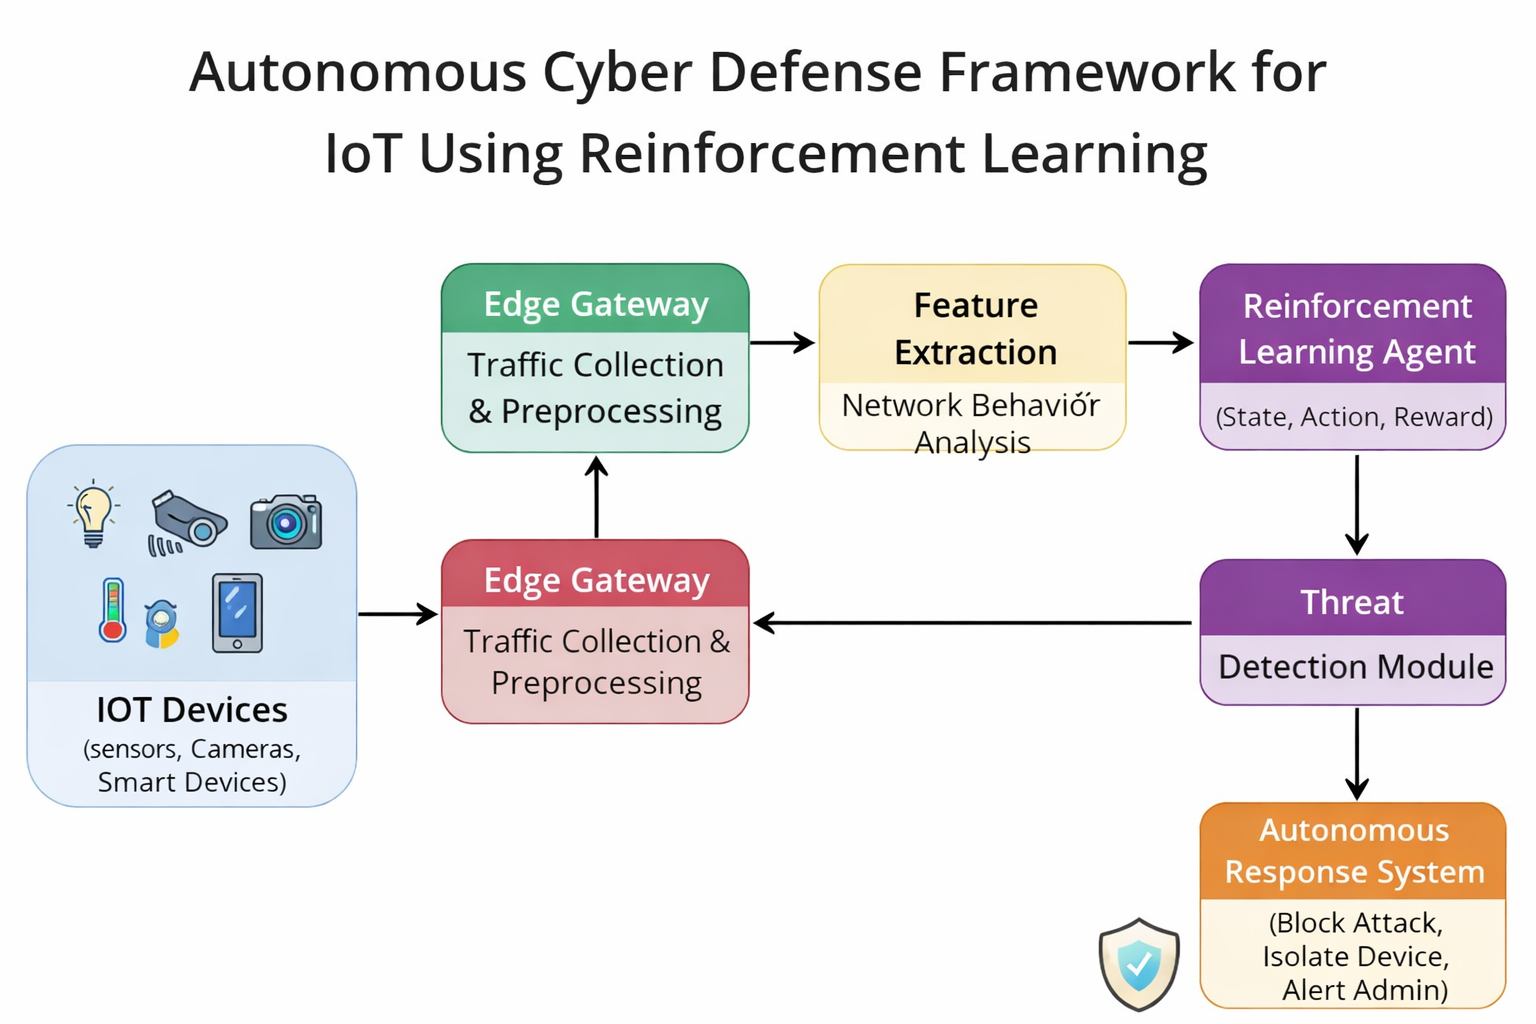
\includegraphics[width=\linewidth]{rl_iot_framework.png}
\caption{Autonomous Cyber Defense Framework for IoT Using Reinforcement Learning}
\label{fig:rl_iot_framework}
\end{figure}

As shown in Fig.~\ref{fig:rl_iot_framework}, the reinforcement learning based cyber defense framework analyzes IoT network traffic and autonomously detects cyber threats.
\subsection{Evaluation Metrics}
Evaluating the capabilities of cybersecurity systems requires the use of appropriate indicators to assess the precision and effectiveness of methods used to detect threats. When discussing Internet of Things (IoT) security, there are various indicators used to assess the capacity of intrusion detection systems and machine learning based defense systems. The indicators enable us to establish quantitative parameters to determine how effectively the proposed reinforcement learning system can identify any malicious activities and provide protection against cyber attacks against the network. 
One important indicator is detection accuracy. Detection accuracy refers to the ratio of correctly identified network events to the total number of network events monitored by the system. Good detection accuracy means that the system is capable of identifying normal network traffic and detecting malicious activities. Although good detection accuracy is important, relying solely on it provides limited information about the effectiveness of a system. 
The false positive rate is another key indicator used to gauge the number of legitimate network activities that have been mistakenly identified as cyber-attacks. A high false positive rate leads to unnecessary alarms and undermines the trustworthiness of a security system. Hence, a good Internet of Things based intrusion detection system must have a low false positive rate along with strong detection accuracy. 
Research on Internet of Things based cyber- security solutions emphasize the need to strike a balance between increasing the detection accuracy and reducing the false positive rate to achieve effective threat detection capability \cite{Cevallos2023, Li2024, Alnfiai2025, Ogenyi2025}
Precision and recall are widely used indicators to measure the capability of a cyber security system. Precision calculates the ratio of correctly detected cyber attacks out of all incidents identified by the system as cyber-attacks. Recall indicates the system's ability to identify actual cyber-attacks that occur within the network. Combined together, we can calculate the F1 Score which provides a comprehensive assessment of our ability to detect attacks. 
In addition, the capacity to respond to cyber threats is a vital indicator to evaluate autonomous cyber defense systems. Response time indicates the speed at which a cyber-defense system can identify and act upon a cyber-attack after it occurs. Reinforcement learning based cyber defense systems aim to minimize the response time through providing automated approaches to counter threats. Fast response times are necessary to contain the spread of cyber attacks in IoT networks.\cite{Brown2024}
\subsection{Experimental Results and Discussion}
The results of the experiment confirm the effectiveness of the RL-based cyber defense system in terms of finding and stopping cyber threats that exist in IoT environments. In the training phase, RL agent continued to improve its ability to find malicious network activity by repeatedly interacting with the Subsystem environment. The increased duration of the training resulted in increased levels of detection and improved capability for handling cyber threats.
The results also indicated that an RL-based intrusion detection system is capable of detecting multiple types of cyberattacks including Denial of Service (DoS), unauthorized access and anomalous device communications. The RL agent was able to use experience from its past interactions to modify its decision-making and consequently enhance its long-term ability to detect cyber threats.
In order to provide protection for an IoT network against new cyber threats that have been previously unidentified or documented, the system must possess exceptional adaptability capabilities.
The proposed RL-based framework achieved improved accuracy and faster response time compared to traditional rule based intrusion detection systems. The RL agent's ability to adaptively modify its defensive strategy provides the capability for the system to respond effectively to new and evolving threats. Similar findings have been reported in other recent RL based cybersecurity studies cited in [23].
The experimental study demonstrated that our proposed system significantly reduces the number of false positives that it generates. The continual improvement in its ability to recognize intrusions is achieved through RL learning and through the continual accumulation of performance data.\cite{Zhang2024, Khan2023, Patel2024, Wang2023, Gupta2024, Sharma2023,Khan2023}

	

	\section{Practical Insights and Use Cases}
	\subsection{Reinforcement Learning for Smart Home Security}
    Smart home technologies have developed tremendously over the past few decades, providing us with a very connected world of sensors, smart appliances, cameras, and voice-enabled devices. This results in constant wireless communication between those devices; each device continuously exchanging data with the others using a wireless connection. Unfortunately, the widespread availability of such connectivity has created many new opportunities for cyber criminals to exploit security weaknesses.



Network security has traditionally been based on standards that were designed for protecting typical computer network environments. Network and device security measures simply cannot provide a level of security comparable to traditional computer network security measures in today's smart home environment. The constraints of IoT devices have produced a need for different security measures than traditional network technologies. The computation capabilities of IoT devices are generally very limited, and their communication patterns change often. Researchers continue to study the potential application of reinforcement learning (RL) techniques to address this need for an adaptive cybersecurity framework that will continuously learn from the network activity of IoT devices and detect suspicious activity in real time.



There are several ways in which RL agents can monitor the network communication traffic generated by the large volume of IoT devices in a smart home. Some examples of the different types of IoT traffic generated by these devices would be smart thermostats, smart lighting systems, surveillance cameras, and smart locks. Patterns of communication generated by each of these IoT devices can be monitored by their respective RL agents, making use of the historical data collected on the various devices' patterns of communication to develop patterns of normal operation for all connected IoT devices. Each of the RL agents continuously monitors each of the IoT devices and their respective communication patterns to detect any irregular communication patterns that might represent an attempt to conduct a cyber-attack. For example, if an IoT device has been compromised and starts sending large amounts of data to an unknown external source, its RL agent will identify that this data transfer is unusual, consider it a possible attack, and initiate a countermeasure. The countermeasure is an automated response to the detected irregular communications.\cite{Ahmed2025, Nguyen2023, Palmer2024, Li2024}
\subsection{Industrial IoT Cyber Defense Applications}
Industrial Internet of Things (IIoT) environments provide areas where robust cybersecurity measures are required. Modern industries employ connected sensors, automated equipment and remote monitoring tools to enhance their capacity to deliver goods and services with increased level of operational efficiency. Even as good level of network connectivity offers several advantages, Industrial Internet of Things technologies are vulnerable to a wide array of cyber threats, including denial of service attacks, viruses/malware and unauthorized access to systems. \cite{Wang2024}
Cyber defense solutions based on reinforcement learning can help to identify and deal with challenges arising due to Industrial IoT.
Industrial automation infrastructures offer good opportunities to implement RL based cyber security measures. Industrial edge gateways or network monitoring systems can be used to train reinforcement learning agents to process large amounts of data coming from industrial sensors and actuators. The Reinforcement Learning Agents can continuously track the network's data flows and identify any differences between normal industrial activities and possible threats. For example, any sudden change in communication between industrial equipment and control systems could indicate an attempt to undermine a factory's ability to produce goods. 
One of the key strengths of Reinforcement Learning in providing security to the industrial internet of things is its ability to enable systems to make decisions independently. If any cyber attack is detected, appropriate defensive measures such as restricting suspicious communication channels, identifying and isolating infected nodes or diverting internet traffic to secure networks with real time monitoring capabilities can be taken.
For industries, delayed action against cyber attacks can lead to losses in production or financial terms. Research studies by Al-Hawawreh et al. and Ullah et al. indicate that Reinforcement Learning based models have a high capacity to detect intruders in Industrial Networks better than traditional Rule Based Systems. Having the ability to identify and adapt to changes in the network and the evolving strategies of hackers, Reinforcement Learning based Defense Systems contribute to creating a robust Cyber Security framework necessary to provide good level of protection to important Industrial Infrastructure.\cite{Alnfiai2025, Ogenyi2025, Jamshidi2025, Khan2023}
\subsection{Cybersecurity in Smart Cities and Critical Infrastructure}
The goal of smart city initiatives is to introduce advanced digital technologies into urban infrastructure to create better transportation systems, manage energy supplies, provide good healthcare facilities and ensure public safety. Such areas require robust large-scale Internet of Things (IoT) networks comprising of thousands of sensors, surveillance cameras, traffic monitoring devices and data communication platforms. Although we have the benefit of advanced technologies for building a better urban life, they also create good challenges related to data security. Providing safe and secure smart city infrastructure requires advanced and effective methods of securing large-scale data networks which can provide real-time cyber threat detection capabilities. 
Reinforcement learning-based cybersecurity solutions provide an effective way to ensure a secure smart city environment. Reinforcement learning agents monitor the network traffic generated by various IoT devices spread across the city and identify any unusual communication pattern indicating a cyber attack like a Distributed Denial of Service (DDoS) attack, Data Tampering attempt or unauthorized access to critical infrastructure system. 
Auto-defence systems enable immediate action to be taken if any suspicious activity is detected. For eg., the system can block malicious internet traffic, isolate infected devices or redirect data streams to centralised security control rooms for detailed analysis. Reinforcing security measures through automatic responses help contain cyber attacks from spreading across inter-linked infrastructure such as transportation systems, smart grids and communication systems used during emergencies. 
Recent studies highlight the need for AI based cybersecurity technologies to build safe and secured Smart City infrastructure. Studies conducted by Zhang et al. and Singh et al. show that Reinforcement Learning based Intrusion Detection Systems offer improved scalability and adaptability compared to traditional ways of providing security. As we see Smart Cities being set up all over the world, applying Reinforcement Learning based Cybersecurity solutions will contribute towards creating a safe, reliable, efficient and resilient urban digital infrastructure.\cite{Zhang2024, Singh2024, Patel2024, Gupta2024, Sharma2023}
	

	\section{Challenges and Open Issues}
	\subsection{Scalability and Resource Constraints in IoT Networks}
    A key challenge in implementing reinforcement learning-based cybersecurity frameworks in Internet of Things (IoT) environments is the challenge of scalability and limited device capabilities. IoT networks comprise a very large number of diverse devices including sensors, actuators, smart gadgets and embedded devices. These devices are equipped with limited computational powers, low storage capacities and restricted energy sources. Consequently, deploying sophisticated machine learning algorithms on these devices is challenging.
The deep reinforcement learning models need substantial computational capacity to learn and make predictions. Large-scale IoT environments dealing with vast amount of network traffic data generated by thousands of devices present further challenges. If we deploy the learning process on IoT devices themselves, it may lead to degraded system performance, increased power consumption and shorter gadget lifespan. Therefore, various research groups suggest employing Edge Computing or Cloud Based architectures to lighten the computing burden from the resource-starved devices. 
Scalability is also a challenge resulting from the dynamic and expansive nature of IoT networks. New devices are added to the network on a continuous basis leading to changes in the overall system behavior and inducing new communication patterns. The Reinforcement Learning Models trained for a specific Network Configuration may fail to adapt to changes in network expansion or when new devices with distinct communication characteristics are added. This can lead to reduced ability to detect intrusions. 
Real-time threat detection in huge IoT networks requires efficient data collection and processing methods. If the system is unable to process network data at required speed, there could be delay in detecting attacks providing opportunities to malicious activities to spread through the network. Addressing challenges related to Scalability is a pressing challenge to develop effective Reinforcement Learning based Cybersecurity Solutions for IoT network environments.\cite{Nguyen2023, Li2024, Palmer2024}
\subsection{Security of Learning Models and Adversarial Attacks}
Although reinforcement learning-based cybersecurity systems provide effective methods to identify various types of cyber threats, the models used for learning can be vulnerable to sophisticated adversarial attacks. Attackers can try to deceive the training data or create vulnerabilities in the learning process in order to bypass the detection mechanisms. Attacks on the learning models can significantly undermine the ability of reinforcement learning-based systems to provide adequate defenses.\cite{Chen2023}
Cyber attacks involving adversarial examples are another concern. Adversarial examples involve modifying network traffic patterns that appear normal to ML models but can enable malicious activities. Carefully crafted input data can confuse reinforcement learning agents and create obstacles for them to identify cyber-attacks effectively. Consequently, malicious activities can continue undetected within a network for extended periods of time.
A potential area of vulnerability is poison attacks, which involve adding malware-ridden data to the training dataset used by reinforcement learning models. If a system is trained using manipulated data, it may develop ineffective methods for identifying cyber threats, allowing attackers to gain better access to the network. Cyber threats through poisoning attacks are a serious issue, especially in Internet of Things (IoT) environments with large numbers of geographically distributed devices providing data, and the challenge of verifying the authenticity of all available data. 
Reinforcement learning based models need to engage in continuous interactions with the network environment to enhance their ability to make effective decisions. During the training phase, hackers can artificially create faulty patterns of behavior to influence the agent's reward function and lead to suboptimal defensive strategies. Enhancing the capacity of learning models to withstand such adversarial attempts at manipulation is an important unsolved challenge in the field of AI-driven Cyber Security.\cite{Ahmed2025,Gupta2024, Alnfiai2025, Ogenyi2025}
\subsection{Privacy, Trust, and Deployment Challenges}
The use of reinforcement learning-enabled cybersecurity models poses significant challenges with regard to privacy and data protection issues in IoT scenarios. IoT devices gather and transfer considerable amounts of information that might consist of such sensitive data as individual behavioral characteristics, health-related statistics, geolocation data, and even data related to industrial operations. For effective cyber threat detection and identification, security solutions require analysis of the network traffic and activity patterns, implying that the analysis involves the use of this sensitive data. Without proper privacy protection, this sensitive data can be leaked. Also, due to the fact that large amounts of data have to be gathered for reinforcement learning model training, the datasets can fall victim to attacks by malicious actors. Thus, it is important to ensure that the security systems are well protected from potential vulnerabilities.\cite{Farooq2025}



An equally significant problem that arises in this respect is one relating to the trust and reliability of the autonomous nature of such cybersecurity systems. Reinforcement learning-based defense algorithms function with a bare minimum of human involvement and depend on automatic decision-making processes for detecting and dealing with cyberattacks. Although such systems enable rapid response to any cyberattacks, this process itself might become an issue because of the lack of transparency and accountability involved in such cases. In case of incorrect classification of benign traffic as malicious by the learning algorithm, there could be a possibility of blocking genuine communication processes or disrupting the functioning of IoT devices. Moreover, the inclusion of intelligent defense algorithms within the current IoT framework might become challenging due to dissimilarities between hardware platforms, communication protocols, and architecture of the system.\cite{Cevallos2023, Khan2023, Sharma2023}
	

	\section{Future Directions}
	\subsection{Federated and Distributed Learning for IoT Security}
    Future research on reinforcement learning based cybersecurity systems for Internet of Things (IoT) environments will focus on developing distributed learning architectures to efficiently manage large-scale IoT deployments. Traditional machine learning approaches rely on centralized training techniques where data from multiple devices is sent to a central server for training and building models. However, in IoT environments, this approach could lead to several challenges such as increased network delays, high communication overheads and potential threats to data privacy. As IoT devices generate huge amounts of data continuously, sending all of it to centralized systems creates limitations in terms of network bandwidth and introduces challenges related to data security. Therefore, researchers are keenly interested in exploring decentralized approaches to enable collaborative model training techniques that reduce the need to transfer data over networks. 
Federated learning presents an opportunity to address these challenges. In federated learning systems, IoT devices or edge devices can build local models using their own data and communicate only the model parameters with a central data aggregator server. The ability to train local models ensures good data privacy as device data is not exposed beyond its local domain. Combining Reinforcement Learning with Federated Learning enables us to develop decentralised cyber security capabilities involving multiple devices working together to detect and counter cyber attacks within a network. Such systems enable us to learn from diverse types of cyber-attacks occurring at various parts of the network, ensuring good data privacy and scalability. Further research avenues include developing efficient communication protocols and dynamic accumulation strategies to enhance the efficiency of Federated Reinforcement Learning techniques for IoT based Cyber Security Systems.\cite{Jamshidi2025, Wang2023, Patel2024}
\subsection{Energy Efficient Reinforcement Learning Models}
Another area of research needed to advance our understanding of the role of artificial intelligence (AI) in the Internet of Things (IoT) is the development of energy-efficient reinforcement learning models capable of operating effectively on resource-constrained IoT devices. Various IoT devices such as sensors, wearables and embedded controllers have limited capabilities in terms of computational power, memory capacity and battery life. Running sophisticated deep learning algorithms on these devices could increase the energy consumed and shorten its operational lifetime. Therefore, hosting large-scale reinforcement learning models on IoT devices is challenging in several real-world applications. It is necessary to create lightweight machine learning models with strong cybersecurity features and minimal computational requirements. 

Researchers are working to improve the effectiveness of AI based cybersecurity systems through various methods. Techniques like model compression (pruning and quantisation) can be used to reduce the size of neural networks without affecting their capabilities. Techniques such as knowledge distillation enable smaller models to benefit from training data of larger models, allowing them to be easily deployed on low power devices. Edge computing infrastructure provides a good option to distribute the compute-intensive tasks to nearby edge servers enabling IoT devices to focus on collecting and communicating data. Combining lightweight models with edge computing capabilities can provide good balance between high level of detection capability and improved energy efficiency through reinforcement learning based security frameworks. Advancements in hardware capabilities and developing efficient algorithms would contribute significantly in making available efficient Cyber Security systems using AI technology for IoT environment.\cite{Li2024, Nguyen2023, Palmer2024}


\subsection{Explainable and Trustworthy AI for Cyber Defense}
As autonomously functioning cybersecurity systems based on Reinforcement Learning increase in capability, creating strong areas of transparency and reliability will be important challenges for future research. Many Artificial Intelligence systems function as complex "black boxes" - indicating that understanding the underlying decision-making processes of such systems is challenging for humans. In Cybersecurity applications, the lack of clarity about system functioning creates challenges for System Administrators who want to understand why some network activities have been identified as malicious. If an autonomous defensive system mistakenly identifies legitimate actions as Cyber attacks, it can lead to disruption of normal network operations or blocking of important communication lines. We need to ensure that all Reinforcement Learning models generate explanations that are interpretable. Enhancing the capabilities of Autonomous Cybersecurity frameworks requires providing interpretable and explainable outputs from Reinforce-ment Learning models. 

The field of Explainable Artificial Intelligence (AI) provides effective tools to address the challenges posed by current AI systems. Integrating elements that provide clarity into Reinforcement Learning models enables us to identify the factors that contribute to detecting cyber threats. Visualization tools and decision explanation models can enable security professionals to identify the basis of machine learning driven automated actions and verify the dependability of a system. Building reliable Artificial Intelligence systems involves enhancing our ability to counter Adversarial Attacks as well as ensuring that our Artificial Intelligence models can provide consistent levels of performance even in dynamic network environments. Studies to combine Explainable AI with Reinforcement Learning techniques can lead to development of advanced Cybersecurity Systems which are intelligent, clear, reliable and easy to implement in critical IoT networks.\cite{Cevallos2023, Gupta2024, Sharma2023}
	

	\section{Conclusion}
	The rapid development of Internet of Things technologies is transforming modern digital infrastructure by providing seamless connectivity options for devices, services and end-users. IoT solutions are being increasingly used in areas such as smart homes, healthcare monitoring systems, industrial automation, transportation systems and smart cities. Although these technologies offer good opportunities to increase our capacities to deal with issues of efficiency, automation and real-time data availability, they present challenges related to cyber security. The large number of connected devices, varied communication protocols and limited processing capacity of several IoT devices create vulnerabilities which can be exploited by cyber attackers. Conventional approaches to cyber security based on static rules and sign-based intrusion detection systems are inadequate to address the dynamic and evolving challenges posed by IoT. 
Therefore, there is increasing focus on incorporating Artificial Intelligence methods, including reinforcement learning, to develop advanced and adaptable solutions to the challenges of cyber security.
This paper looks at the role played by reinforcement learning in creating autonomous systems to secure IoT ecosystems. Reinforcement learning enables intelligent entities to find effective ways to deal with security challenges through interactions with the network environment and enhancing their capability to make decisions through continuous learning. Through studying network traffic patterns, identifying anomalies and responding to any suspicious activity, reinforcement learning based network intrusion detection systems can improve the ability of IoT networks to identify and counter cyber attacks in real time. The paper also discusses various types of network architectures and application domains where reinforcement learning based security solutions can be applied, such as securing smart homes, providing industrial IoT security and monitoring the intelligent infrastructure of smart cities. These applications highlight the capacity to create autonomous cyber security systems to enhance the capability of large scale IoT deployments to withstand and cope with disruptions.

Although reinforcement learning driven cybersecurity systems offer some benefits, challenges and areas requiring further study remain. IoT systems include devices with limited capabilities to process information, store data and provide necessary energy resources. Providing these complex deep reinforcement learning models with sufficient capability to operate effectively in such devices is challenging unless they are supported by edge computing technology or distributed learning architecture. Moreover, machine learning based cybersecurity systems themselves could be vulnerable to cyber attacks (known as "adversarial attacks") where malicious entities aim to manipulate the training data of AI/ML models or exploit any vulnerabilities in these models. Concerns about data protection, system transparency and building trust in AI/ ML-based automated decision-making systems create barriers to widespread deployment of Artificial Intelligence (AI) based Cybersecurity Systems. 
Future research directions focus on creating effective and efficient Machine Learning (ML) architectures to deal with increasing complexities of IoT ecosystems. Technologies such as Federated Learning, compact Reinforcement Learning Models and Explainable Artificial Intelligence can be used to address several challenges associated with IoT ecosystem management. Enhancing the level of model transparency and ensuring good data governance practices can contribute to building trust in Automated Cyber Security Systems. As IoT technologies evolve and get deeply integrated with critical infrastructure systems, developing Intelligent, Adaptive and Reliable Cyber Defense Mechanisms will remain a crucial challenge. Hence, Reinforcement Learning based Cyber Security Frameworks serve as a significant tool to build robust and Secure IoT Ecosystems which can defend against sophisticated cyber threats.
	

	\bibliographystyle{plain}
	\bibliography{references}
	
\end{document}
